\section{Approach for Decomposition and Collaboration} 
The Fig.\ref{fig_approach} shows the whole framework of decomposing the complete system model to some collaborated sub-systems corresponding. In our research, we implement the decomposition and collaboration algorithms in a tool. In this section, we mainly introduce how we can get the approach of decomposition within resource constraints.

%\TODO{TODO}{repalce the picture Fig 1}

\begin{figure}[!hpbt]
    \centering
        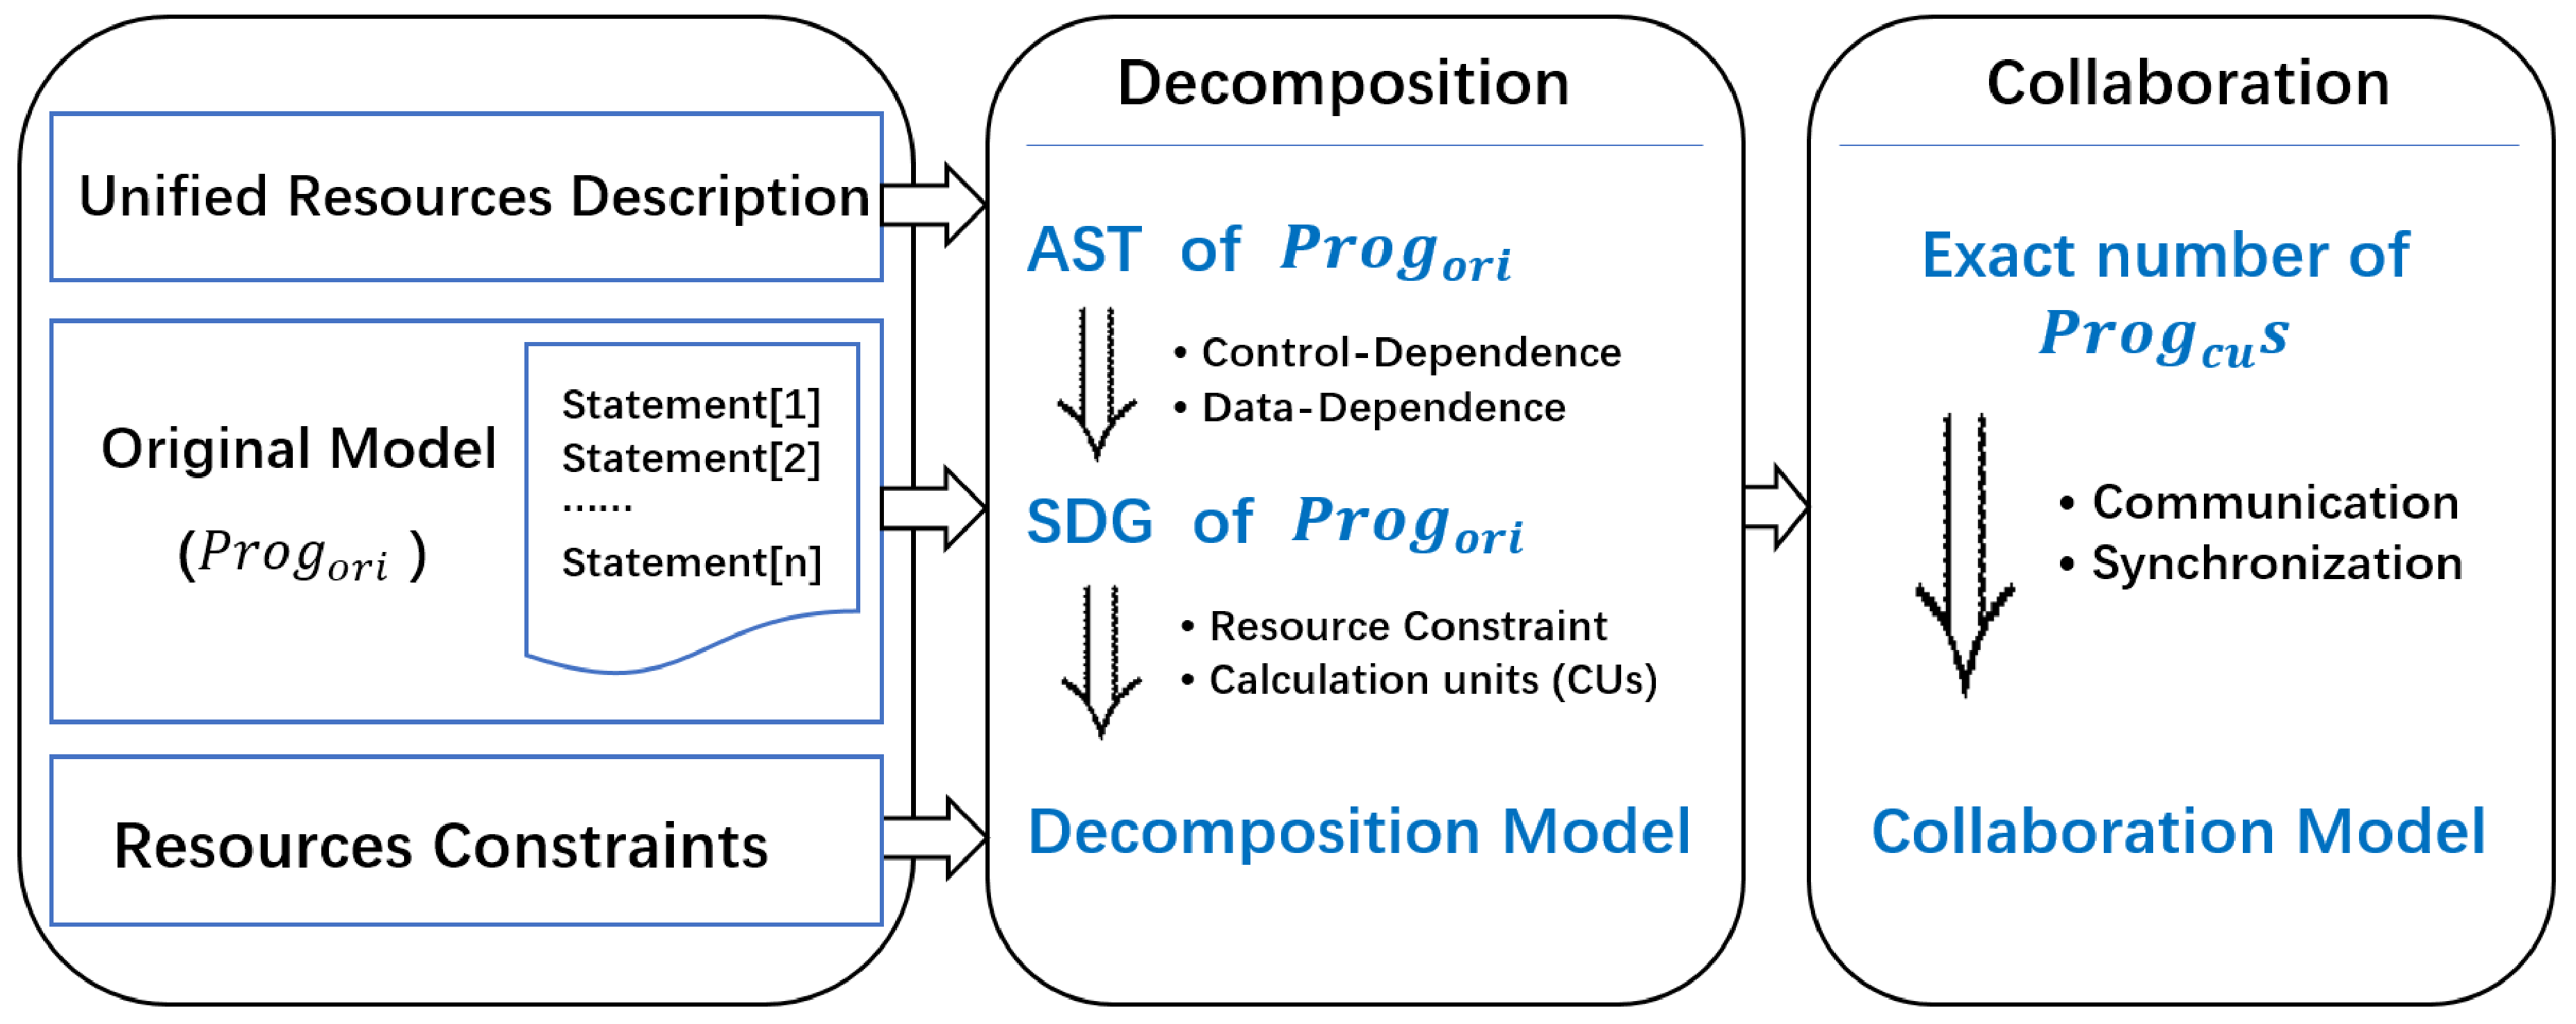
\includegraphics[height=1.4in, width=4.2in]{fig_Approach}
    \caption{Overview of approach for decomposition and collaboration }\label{fig_approach}
\end{figure}

\begin{itemize}
  \item \textbf{Original Model:}\  The Original model is an IMCL program $Prog_{ori}$ given at the beginning time, which is the description of an industrial system.
  \item \textbf{Statement:}\ The $statement$ is the minimum computational task level for the program. Therefore, the $Prog_{ori}$ can be treated as a set of statements.
  \item \textbf{Decomposition Model:}\  It is the multiple models that all of the statements in \emph{Original Model} are decompose to specified $CU$. In other words, it is transformed from a $Prog_{ori}$ under the resources constraint to the set of $Prog_{cu}$ for every \emph{CU}.
  \item \textbf{Collaboration Models:}\  Which is a set of the $Prog_{cu}$ interact with each other with communication and synchronization.
\end{itemize} 